%%%%%%%%%%%%%%%%%%%%%%%%%%%%%%%%%%%%%%%%%
% Short Sectioned Assignment
% LaTeX Template
% Version 1.0 (5/5/12)
%
% This template has been downloaded from:
% http://www.LaTeXTemplates.com
%
% Original author:
% Frits Wenneker (http://www.howtotex.com)
%
% License:
% CC BY-NC-SA 3.0 (http://creativecommons.org/licenses/by-nc-sa/3.0/)
%
%%%%%%%%%%%%%%%%%%%%%%%%%%%%%%%%%%%%%%%%%

%----------------------------------------------------------------------------------------
%	PACKAGES AND OTHER DOCUMENT CONFIGURATIONS
%----------------------------------------------------------------------------------------

\documentclass[paper=a4, fontsize=11pt]{scrartcl} % A4 paper and 11pt font size

\usepackage{tikz}
\usepackage[T1]{fontenc} % Use 8-bit encoding that has 256 glyphs
%\usepackage{fourier} % Use the Adobe Utopia font for the document - comment this line to return to the LaTeX default


\usepackage[american]{babel} % English language/hyphenation
\usepackage{amsmath,amsfonts,amsthm} % Math packages
\usepackage{bm}

\usepackage{csquotes}
\usepackage[style=apa,sortcites=true,sorting=nyt,backend=biber]{biblatex} %bibliography package
\DeclareLanguageMapping{american}{american-apa}
\nocite{*}

\usepackage{sectsty} % Allows customizing section commands
\allsectionsfont{\centering \normalfont\scshape} % Make all sections centered, the default font and small caps

\usepackage{fancyhdr} % Custom headers and footers
\usepackage{outlines}
\usepackage{enumitem}

\pagestyle{fancyplain} % Makes all pages in the document conform to the custom headers and footers
\fancyhead{} % No page header - if you want one, create it in the same way as the footers below
\fancyfoot[L]{} % Empty left footer
\fancyfoot[C]{} % Empty center footer
\fancyfoot[R]{\thepage} % Page numbering for right footer
\renewcommand{\headrulewidth}{0pt} % Remove header underlines
\renewcommand{\footrulewidth}{0pt} % Remove footer underlines
\setlength{\headheight}{13.6pt} % Customize the height of the header

\numberwithin{equation}{section} % Number equations within sections (i.e. 1.1, 1.2, 2.1, 2.2 instead of 1, 2, 3, 4)
\numberwithin{figure}{section} % Number figures within sections (i.e. 1.1, 1.2, 2.1, 2.2 instead of 1, 2, 3, 4)
\numberwithin{table}{section} % Number tables within sections (i.e. 1.1, 1.2, 2.1, 2.2 instead of 1, 2, 3, 4)

\setlength\parindent{0pt} % Removes all indentation from paragraphs - comment this line for an assignment with lots of text

\bibliography{biblio}
%----------------------------------------------------------------------------------------
%	TITLE SECTION
%----------------------------------------------------------------------------------------

\newcommand{\horrule}[1]{\rule{\linewidth}{#1}} % Create horizontal rule command with 1 argument of height

\title{	
\normalfont \normalsize 
\textsc{Math 460} \\ [25pt] % Your university, school and/or department name(s)
\horrule{0.5pt} \\[0.4cm] % Thin top horizontal rule
\huge Golay Codes\\ % The assignment title
\horrule{2pt} \\[0.5cm] % Thick bottom horizontal rule
}

\author{Dean Bisogno} % Your name

\date{\normalsize\today} % Today's date or a custom date
\newtheorem{defn}{Definition}
\newtheorem{thm}{Theorem}
\newtheorem{lma}{Lemma}
\setenumerate[1]{label=\Roman*.}
\setenumerate[2]{label=\Alph*.}
\setenumerate[3]{label=\roman*.}
\setenumerate[4]{label=\alph*.}

\begin{document}
\maketitle % Print the title

\section{History and Constructions}

The Golay code developed by Marcel Golay in 1949 has had significant impact on the advancement of coding theory, the classification of simple finite groups, and communication systems. Golay's 1949 article ``Notes on Digital Coding'' appeared in the June edition of the Proceedings of the IRE [\cite{golay}]. In ``Notes on Digital Coding'' Golay presented a generalization of the Hamming(7,4) code which he had read about in Shannon's 1948 paper. After generalizing the perfect, single error-correcting codes, Golay then justifies the existence of two codes which can correct multiple errors, the perfect binary Golay code $\mathcal{G}_{23}$, and the ternary Golay code. At the bottom of the article Golay supplied generator matrices for his codes, but lacked any explanation of their construction. Golay would provide explanation of his matrices' construction in 1954. Though brief and without significant justification, Berlekamp called the article ``the best single published page'' and Zaremba once told Golay that he had ``said more in half a page than others have said in twenty pages'' [\cite{thompson}]. The remainder of this section will focus on constructions of $\mathcal{G}_{23}$, $\mathcal{G}_{24}$, and some interesting properties they satisfy. With these constructions and their properties in hand, we will then be able to motivate the study of the Golay codes as Steiner systems with known automorphism groups.

\subsection{Important Definitions}
We first need to equip ourselves with the primitive definitions used when discussing linear codes.

\begin{defn}[linear code and their properties]
A linear code $\mathcal{C}$ is a subspace of a vector space $V$. We define the following properties:
\begin{enumerate}
\item \textit{length}: the number of characters, $n$, in a word in $\mathcal{C}$.
\item \textit{dimension}: the number of characters, $k$, which uniquely determine a word in $\mathcal{C}$.
\item \textit{distance}: the number of positions, $d$ in which two words differ.
\item \textit{weight}: the number of positions in which a word differs from the zero word.
\item \textit{detectable errors}: the number of errors a code can detect is $d-1$.
\item \textit{correctable errors}: the number of errors a code can correct is $t=\lfloor \frac{d-1}{2} \rfloor$.
\end{enumerate} 
\end{defn}

For a linear code, the minimum weight will coincide with the minimum distance. This is trivial to see since $\mathcal{C}$ is a vector subspace, it is closed under vector addition. Thus if any two vectors $\bf{v}$,$\bf{w}$ have the minimum distance between them, then $\bf{v}-\bf{v}=\bf{0}$ and $\bf{w}-\bf{v}$ are separated by the same distance.

\begin{defn}[perfect]
A code $\mathcal{C}$ with minimum weight $d$ in a vector space $V$ is \textit{perfect} if all the vectors in $V$ are contained in spheres of radius $r=\lfloor \frac{d-1}{2} \rfloor$ centered around the codewords. We note that $r$ corresponds to the definition of the code's correctable number of errors.
\end{defn}

The Hamming (7,4,3) codes present such a partition of $(\mathbb{Z}/2)^7$ as we can show. Consider an arbitrary $c \in \mathcal{C}$. Then the number of vectors in a sphere of radius 1 centered at $c$ is
$$
V_1(c) = \#{x | d(x,c)\leq 1} = {7 \choose 1} + {7 \choose 0} = 8 = 2^3
$$

And since $|\mathcal{C}|= 2^4$ we have $2^4 \cdot 2^3 = 2^7=|(\mathbb{Z}/2)^7|$. Which shows that spheres with radius $r = \lfloor \frac{3-1}{2} \rfloor$ centered at codewords partitions $\mathbb{Z}/2)^7$. This example motivates the following theorem which we will use to restrict where we expect perfect codes to exist.

\begin{thm}[\cite{pless}]
In order for a perfect $t$-error-correcting [$n$,$k$] code over $GF(q)$ to exist we require that
$$
q^k ({n \choose 0} +  \sum_{i=1}^t ((q-1)^i{n \choose i}) = q^n. 
$$
\end{thm}

This places necessary, but not sufficient, conditions on $n$,$t$, and $k$. To find his codes Golay used Pascal's triangle and indexed the rows by $n = 0, 1, \ldots$ and the position of each element on its row by $t = 0,1, \ldots$. Then for a row $n$ if the first $t \geq 3$ elements of a row sum to a power $k$ of $q$, we suspect an [$n$,$k$] $t$-error-correcting code may exist. We will see a more explicit application in the next section where we will construct the perfect $\mathcal{G}_{23}$ which is a [23,11] 3-error-correcting code.
%Then we can motivate the Golay Codes as steiner systems which we can show to be unique and equipped with known automorphism groups. These connections are the tools that allowed $\mathcal{G}_{24}$ to be used in the classification of finite simple groups and in particular aided in the discovery of Conway's sporadic groups $Co_1$,$Co_2$, and $Co_3$ [\cite{thompson}]. 
\subsection{Constructions of $\mathcal{G}_{23}$}
This section will concentrate on Golay's original construction of $\mathcal{G}_{23}$. First let us define what we are looking for.
Golay first used Pascal's triangle to find 3 binomial coefficients which summed to a power of 2. The 23rd row of Pascal's triangle indicates that
$$\sum_{i=0}^3 {23 \choose i} = 1+23+253+1771 = 2048 = 2^{11}$$. This tell us that on the 23-cube, a sphere with Hamming radius atleast 3 contains a number of vertices which divides $2^{23}$ i.e. $V(S_{\geq 3}(x) )|2^{23}$ where $x$ is a vertex of the 23-cube. This implies that the minimum weight of $\mathcal{G}_{23}$ must be equal to $2*3+1=7$. Without justification Golay provided the generator matrix $\mathbf{A}$ for $\mathcal{G}_{23}$:

$$\textbf{A} = \begin{array}{ccccccccccccc}
& Y_1 & Y_2 & Y_3 & Y_4 & Y_5 & Y_6 & Y_7 & Y_8 & Y_9 & Y_{10} & Y_{11} & Y_{12} \\
   X_1 & 1 & 0 & 0 & 1 & 1 & 1 & 0 & 0 & 0 & 1 & 1 & 1\\
   X_2 & 1 & 0 & 1 & 0 & 1 & 1 & 0 & 1 & 1 & 0 & 0 & 1\\
   X_3 & 1 & 0 & 1 & 1 & 0 & 1 & 1 & 0 & 1 & 0 & 1 & 0\\
   X_4 & 1 & 0 & 1 & 1 & 1 & 0 & 1 & 1 & 0 & 1 & 0 & 0\\
   X_5 & 1 & 1 & 0 & 0 & 1 & 1 & 1 & 0 & 1 & 1 & 0 & 0\\
   X_6 & 1 & 1 & 0 & 1 & 0 & 1 & 1 & 1 & 0 & 0 & 0 & 1\\
   X_7 & 1 & 1 & 0 & 1 & 1 & 0 & 0 & 1 & 1 & 0 & 1 & 0\\
   X_8 & 1 & 1 & 1 & 0 & 0 & 1 & 0 & 1 & 0 & 1 & 1 & 0\\
   X_9 & 1 & 1 & 1 & 0 & 1 & 0 & 1 & 0 & 0 & 0 & 1 & 1\\
X_{10} & 1 & 1 & 1 & 1 & 0 & 0 & 0 & 0 & 1 & 1 & 0 & 1\\
X_{11} & 0 & 1 & 1 & 1 & 1 & 1 & 1 & 1 & 1 & 1 & 1 & 1\\
\end{array}$$
Using this matrix we can map data vectors in $(\mathbb{Z}/2)^{12}$ to parity check words in $(\mathbb{Z}/2)^{11}$. Then for a data vector $\mathbf{v} \in (\mathbb{Z}/2)^{23}$ we can build the message $\mathbf{m} = (\mathbf{v},\mathbf{A}\mathbf{v})$. The parity check matrix is then $[\mathbf{A}:\mathbf{I}_{11}]$, and is a linear transformation $$[\mathbf{A}:\mathbf{I}_{11}]: (\mathbb{Z}/2)^{23} \longrightarrow (\mathbb{Z}/2)^{11},$$ where $\mathcal{G}_{23}=Ker([\mathbf{A}:\mathbf{I}_{11}])$. Thus to check to see if a received message $\mathbf{m}$ has an error we just check $\mathbf{Pm} \equiv 0 (mod 2)$.

The construction given by Golay for matrix $\textbf{A}$ depends upon a sketch of five lines.

\begin{figure}[!ht]
  \centering
  \def\svgwidth{150pt}
  \input{lines.pdf_tex}  
  \caption{Golay's lines}
  \label{fig:cstori}
\end{figure}

Then we label the minor matrix consisting of rows $X_1 \ldots X_{10}$ and columns $Y_2 \ldots Y_{12}$.

$$\textbf{A} = \begin{array}{ccccccccccccc}
&&       A  &  B  &  C  &  D  &  E &\sigma_1&\sigma_2&\sigma_3&\sigma_4&\sigma_5&\sigma_6\\
&&      Y_2 & Y_3 & Y_4 & Y_5 & Y_6 & Y_7 & Y_8 & Y_9 & Y_{10} & Y_{11} & Y_{12} \\
AB &    X_1 & 0 & 0 & 1 & 1 & 1 & 0 & 0 & 0 & 1 & 1 & 1\\
AC &    X_2 & 0 & 1 & 0 & 1 & 1 & 0 & 1 & 1 & 0 & 0 & 1\\
AD &    X_3 & 0 & 1 & 1 & 0 & 1 & 1 & 0 & 1 & 0 & 1 & 0\\
AE &    X_4 & 0 & 1 & 1 & 1 & 0 & 1 & 1 & 0 & 1 & 0 & 0\\
BC &    X_5 & 1 & 0 & 0 & 1 & 1 & 1 & 0 & 1 & 1 & 0 & 0\\
BD &    X_6 & 1 & 0 & 1 & 0 & 1 & 1 & 1 & 0 & 0 & 0 & 1\\
BE &    X_7 & 1 & 0 & 1 & 1 & 0 & 0 & 1 & 1 & 0 & 1 & 0\\
CD &    X_8 & 1 & 1 & 0 & 0 & 1 & 0 & 1 & 0 & 1 & 1 & 0\\
CE &    X_9 & 1 & 1 & 0 & 1 & 0 & 1 & 0 & 0 & 0 & 1 & 1\\
DE & X_{10} & 1 & 1 & 1 & 0 & 0 & 0 & 0 & 1 & 1 & 0 & 1\\
\end{array}$$
$$\sigma_1=(ABEDC), \sigma_2=(ABCED), \sigma_3=(ABDCE),$$
$$\sigma_4=(ACEBD), \sigma_5=(ACBDE), \sigma_6=(ADCBE)$$
Then for columns $Y_2 \ldots Y_6$ we place a 0 in the rows corresponding to intersections with the respective line, and 1 otherwise. In columns $Y_6 \ldots Y_{12}$ we place 0's in the rows where the corresponding transposition appears in the cycle, and ones elsewhere. The resulting matrix has rows and columns of minimum weight 6, so 
$$Y_1 = [ \begin{array}{ccccccccccc} 1& 1& 1& 1& 1& 1& 1& 1& 1& 1& 0\end{array}]^T$$
$$X_{12} = [\begin{array}{cccccccccccc} 0& 1& 1& 1& 1& 1& 1& 1& 1& 1\end{array}]$$ fixes the minimum weight to 7 [\cite{thompson}]. To construct $\mathcal{G}_{24}$ we append a 1 to each codeword of odd weight in $mathcal{G}_{23}$ and a zero to all codewords of even weight. This increases the minimum weight to 8, so while the code is no longer perfect, it can detect 7 errors rather than the 6 detectable by $\mathcal{G}_{23}$.

While the above recounts Golay's original construction of the generator matrix of $G_{23}$, history has demonstrated that the $G_{24}$ code is much more useful and more intuitive constructions of either code are available.

\subsection{As a Cyclic Code} (might cut this section)
We can construct $\mathcal{G}_{23}$ more easily by considering the factors of $$x^{23}-1=(x+1)(x^{11}+x^9+x^7+x^6+x^5+x+1)(x^{11}+x^{10}+x^6+x^5+x^4+x^2+1)$$ over $\mathbb{Z}/2$. If we consider $p(x)=x^{11}+x^9+x^7+x^6+x^5+x+1$ (though either degree 11 factor will generate the same code), then we know since $p|x^{23}-1$, that $<p(x)>$ is an ideal in the ring $\mathbb{Z}/2[x]$. Then $<p(x)>$ is closed under multiplication, in particular for any $g(x)\in<p(x)>$, we know $x*g(x)\in<p(x)>$. Further, in $\mathbb{Z}/2[x]$, multiplication by $x$ corresponds to the shift operator. The corresponding matrix for this code is 
$$\textbf{G} = \begin{array}{ccccccccccccc}
       p(x) & 1 & 0 & 1 & 0 & 1 & 1 & 1 & 0 & 0 & 0 & 1 & 1\\
   x^1*p(x) & 1 & 1 & 0 & 1 & 0 & 1 & 1 & 1 & 0 & 0 & 0 & 1\\
   x^2*p(x) & 1 & 1 & 1 & 0 & 1 & 0 & 1 & 1 & 1 & 0 & 0 & 0\\
   x^3*p(x) & 0 & 1 & 1 & 1 & 0 & 1 & 0 & 1 & 1 & 1 & 0 & 0\\
   x^4*p(x) & 0 & 0 & 1 & 1 & 1 & 0 & 1 & 0 & 1 & 1 & 1 & 0\\
   x^5*p(x) & 0 & 0 & 0 & 1 & 1 & 1 & 0 & 1 & 0 & 1 & 1 & 1\\
   x^6*p(x) & 1 & 0 & 0 & 0 & 1 & 1 & 1 & 0 & 1 & 0 & 1 & 1\\
   x^7*p(x) & 1 & 1 & 0 & 0 & 0 & 1 & 1 & 1 & 0 & 1 & 0 & 1\\
   x^8*p(x) & 1 & 1 & 1 & 0 & 0 & 0 & 1 & 1 & 0 & 0 & 1 & 0\\
   x^9*p(x) & 0 & 1 & 1 & 1 & 0 & 0 & 0 & 1 & 1 & 0 & 0 & 1\\
x^{10}*p(x) & 1 & 0 & 1 & 1 & 1 & 0 & 0 & 0 & 1 & 1 & 0 & 0\\
\end{array}$$

\subsection{As a Steiner System}
This is one of the most interesting constructions of the Golay code as it uses particular properties of the code to show that it satisfies the Assmus-Mattson Theorem which proves the existence of the Steiner system construction. Once we know that our construction is valid, we can use properties of Steiner systems to prove the uniqueness of the Golay code and to identify the automorphism group of the $\mathcal{G}_{24}$ code.

\begin{defn}
Consider integers $1 \leq t < k < v$ and $\lambda$. The design $t-(k,v,\lambda)$ is a pair of sets $(\mathfrak{X},\mathfrak{B})$ where $|\mathfrak{X}|=v$ and $\mathfrak{B}$ contains size $k$ subsets of $\mathfrak{X}$, called `blocks,' such that every size $t$ subset of $\mathfrak{X}$ is contained in exactly $\lambda$ blocks. In the particular case that $\lambda=1$, we call it a \textit{Steiner system} S(t,k,v).
\end{defn}

The Fano plane is the geometry associated with S(2,3,7). Seven lines partition the seven points, where each line contains exactly three points, and each pair of points uniquely designates a line.

\begin{figure}[hbp]
\centering
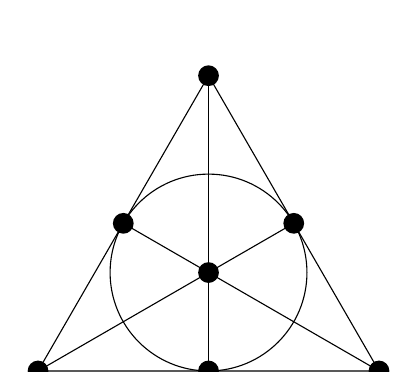
\begin{tikzpicture}[scale=2.5]

   \draw (0,0) circle (0.5);
   \draw (90:1) -- (-30:1)--(210:1)--cycle;

   \draw (90:1)--(0,0);
   \draw (210:1)--(0,0);
   \draw (-30:1)--(0,0);

   \draw (30:0.5)--(0,0);
   \draw (150:0.5)--(0,0);
   \draw (270:0.5)--(0,0);

   \fill (-0.866,-0.5) circle (1.5pt);
   \fill (0.866,-0.5) circle (1.5pt);
   \fill (0,-0.5) circle (1.5pt);
   \fill (0,1) circle (1.5pt);
   \fill (0,0) circle (1.5pt);
   \fill (0.433,0.25) circle (1.5pt);
   \fill (-0.433,0.25) circle (1.5pt);

\end{tikzpicture}
\caption{Fano Plane S(2,3,7)} \label{fig:fplane}
\end{figure}

In particular we want to use the Assmus-Mattson theorem to find the designs corrsponding to the Golay codes. Doing so will require several definitions.
\begin{defn}
Suppose $\mathcal{C}$ is a linear code in vectorspace $V$. We denote 
$$\mathcal{C}^* = \{ \bm{u} \in V | \bm{u} \cdot \bm{w} = 0 \; \forall \; \bm{w} \in V \}. $$
If $\mathcal{C}$ is an $[n,k]$ code, then $\mathcal{C}^*$ is an $[n,n-k]$ code.
Furthermore, if $\mathcal{C}\subseteq\mathcal{C}^*$ then we call $\mathcal{C}$ \textit{totally singular}.
\end{defn}
We note that $\mathcal{G}_{24}$ is totally singular, because the rows of its generator matrix are orthogonal.
More explicitely $\bm{r}_i \cdot \bm{r}_j$ = 0 for any two rows in the matrix $\bm{A}$ of the generator matrix $[\bm{I}_{12}:\bm{A}]$ above. This implies $\mathcal{G}_{24} \subseteq \mathcal{G}_{24}^*$.
\begin{defn}
If $\mathcal{C}$ is totally singular and $dim(\mathcal{C})=\frac{dim(V)}{2}$ then we can $\mathcal{C}$ is \textit{self-dual}.
\end{defn}
We just showed that $\mathcal{G}_{24}$ is totally singular, and we already know that $dim(\mathcal{G}_{24}) = 12 = \frac{24}/2$, so $\mathcal{G}_{24}$ is self-dual.
\begin{defn}[We might not need this definition]
A code $\mathcal{C}$ is \textit{double-even} if for every $x\in \mathcal{C}$, the weight of $c$ is divisible by 4.
\end{defn}
\begin{thm}
Let $\mathcal{C}$ be an $[n,k,d]$ binary code, and let $0<t<d$. Let $B_i$ be the number of vectors of weight $i$ in $\mathcal{C}^*$, and let
$$
s = |{i|B_i \not= 0 \; \& \; 0<i\leq n-t}|.
$$
If $s\leq d-t$, then the vectors of weight $d$ in $\mathcal{C}$ hold a t-design and the vectors of any weight $i\leq n-t$ and $B_i\not=0$ hold a t-design.
\end{thm}

As we've shown that $\mathcal{G}_{24}=\mathcal{G}_{24}^*$, and we know that we can correct 3 errors in any weight 8 word. We are motived to show that $\mathcal{G}_{24}$ contains a $5-(8,24,1)$ design. Since, all vectors in $\mathcal{G}_{24}$ are of weight 8, 12, or 16, we know that $s=3 \leq 8-5$. So the weight eight words contain the Steiner system S(5,8,24). Similar systems can be identified for code words of weight 12 and 16 [\cite{pless}]. 

\section{Uniqueness of $\mathcal{G}_{24}$}
This section will briefly cover the uniqueness proof of $\mathcal{G}_{24}$, these are important as they show that our three constructions actually generate the same code.
\section{The Automorphism Group of $\mathcal{G}_{24}$, $M_{24}$}
Knowing that our constructions are all equiavlent, we can leverage how $\mathcal{G}_{24}$ behaves under $M_{24}$. The Steiner system construction is important here because $M_{24}$ was first understood as the automorphism group of S(5,8,24).

\clearpage
\printbibliography
%----------------------------------------------------------------------------------------

\end{document}